\documentclass{standalone} 
\usepackage{tikz}
\usepackage{graphicx}
\begin{document}
\begin{tikzpicture}
\draw (0,0) grid (11,6);
\fill (2,5) rectangle +(1, 1);
\fill (3,5) rectangle +(1, 1);
\fill (1,4) rectangle +(1, 1);
\fill (4,4) rectangle +(1, 1);
\fill (6,4) rectangle +(1, 1);
\fill (8,4) rectangle +(1, 1);
\fill (9,4) rectangle +(1, 1);
\fill (2,3) rectangle +(1, 1);
\fill (4,3) rectangle +(1, 1);
\fill (6,3) rectangle +(1, 1);
\fill (10,3) rectangle +(1, 1);
\fill (1,2) rectangle +(1, 1);
\fill (3,2) rectangle +(1, 1);
\fill (7,2) rectangle +(1, 1);
\fill (8,2) rectangle +(1, 1);
\fill (3,1) rectangle +(1, 1);
\fill (5,1) rectangle +(1, 1);
\fill (9,1) rectangle +(1, 1);
\fill (1,0) rectangle +(1, 1);
\fill (8,0) rectangle +(1, 1);
\node at (.5, 5.5) {
\includegraphics[width=.9cm]{rato}};
\node at (10.5, .5) {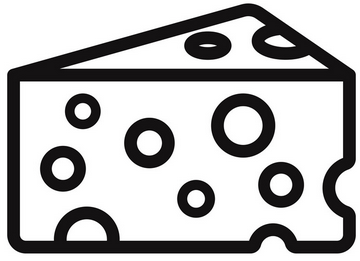
\includegraphics[width=.9cm]{queijo}};
\end{tikzpicture}
\end{document}
